\documentclass{article}

% Recommended, but optional, packages for figures and better typesetting:
\usepackage{microtype}
\usepackage{graphicx}
\usepackage{subfigure}
\usepackage{booktabs} % for professional tables

% hyperref makes hyperlinks in the resulting PDF.
% If your build breaks (sometimes temporarily if a hyperlink spans a page)
% please comment out the following usepackage line and replace
% \usepackage{icml2021} with \usepackage[nohyperref]{icml2021} above.
\usepackage{hyperref}

% Attempt to make hyperref and algorithmic work together better:
\newcommand{\theHalgorithm}{\arabic{algorithm}}

% Use the following line for the initial blind version submitted for review:
%\usepackage{icml2021}

% If accepted, instead use the following line for the camera-ready submission:
\usepackage[accepted]{icml2021}

\begin{document}

\twocolumn[
\icmltitle{Your Full Project Title Here}

\begin{icmlauthorlist}
\icmlauthor{Author One}{}
\icmlauthor{Author Two}{}
\icmlauthor{Author Three}{}
\end{icmlauthorlist}

\vskip 0.3in
]

\section{Process}
In this section, we will discuss our works, explorations, and iterations that led to the final solution. 

\subsection{Data Pre-processing: From Naive Imputation to Stratified Strategy}
Initially, we implemented a naive imputation strategy by replacing all missing values with the feature mean. However, iterative diagnostics revealed that this approach violated the underlying statistical logic, as extreme outliers frequently pulled the mean away from the true central tendency. 

To resolve this, we transitioned to a skewness-based imputation mechanism: features with an absolute skewness greater than 1.0 were imputed with the median, while roughly symmetric features retained mean imputation. For categorical data, we moved beyond uniform mode imputation by incorporating domain-specific insights. We observed that high missing rates often signaled the physical absence of a facility (e.g., "No Basement") rather than random omission . Consequently, we pivoted to imputing "None" for facility-related features and reserved mode imputation only for specific features like \texttt{Electrical}, where missingness was diagnosed as a random human error due to its extremely low frequency and high class dominance.

\subsection{Model Evolution: Overcoming Baseline Pathologies}

Our modeling process was highly iterative, driven by diagnosing and resolving successive algorithmic pathologies. We established our initial baseline using unregularized Ordinary Least Squares (OLS) regression. Instead of standard errors, we observed a catastrophic failure in predictive stability, yielding a sub-optimal $R^2$ score of 0.6797 and violent RMSE fluctuations across cross-validation folds. 

By visualizing the coefficient weights, we discovered a severe case of algorithmic hijacking caused by highly collinear categorical variables. The OLS model created "predictive landmines" by assigning extreme negative weights (e.g., -3.6571) to sparse configurations. Lacking a penalty term, it suffered from perfect multicollinearity, arbitrarily distributing identical weights across related \texttt{\_None} features. 

Diagnosing this pathological behavior provided the definitive mathematical justification for our transition to regularized models (Lasso and Ridge). While L1 and L2 penalties successfully collapsed the inflated multicollinear weights, they introduced a new vulnerability: extreme sensitivity to feature scales and skewness, which we ultimately resolved using the Yeo-Johnson transformation. 

However, even after stabilizing the linear baselines, we recognized a fundamental limitation: linear models cannot inherently capture complex, non-linear interactions between housing features (e.g., the compounding value of high overall quality in a premium neighborhood). This realization catalyzed our architectural pivot to the Gradient Boosting Regressor (GBR). By utilizing an ensemble of decision trees, GBR fundamentally bypassed the multicollinearity trap, required less rigid assumptions about data distribution, and successfully captured the non-linear nuances of the real estate market. Ultimately, this successful transition from linear frameworks to tree-based ensembles not only improved predictive stability but also laid a robust foundation for our subsequent deployment of advanced algorithms, including XGBoost and Stacking architectures.


\subsection{Feature Transformation: Resolving Weight Distortion}
Upon applying regularized linear models (Lasso and Ridge), we observed a stark discrepancy in feature importance compared to our Gradient Boosting Regressor (GBR). The unstandardized linear models disproportionately inflated the weights of one-hot encoded categorical features, such as \texttt{Neighborhood}. In contrast, GBR logically prioritized fundamental structural metrics like \texttt{OverallQual} and \texttt{GrLivArea}.

We diagnosed this as a scale-induced distortion: because one-hot features are bounded between 0 and 1, the linear models assigned them massive coefficients to capture their impact on the target variable. To unify the scales, we initially applied standard scaling (\texttt{StandardScaler}). Surprisingly, this degraded the models' predictive performance. Further investigation revealed that standard scaling failed to correct the underlying high skewness of our numerical features, which violated the homoscedasticity assumption of linear models. 

To resolve both the scale disparity and the non-normality, we implemented a significant engineering pivot by introducing the \textbf{Yeo-Johnson power transformation}. This robust technique successfully normalized highly skewed features while standardizing their scales. Consequently, the predictive accuracy of our regularized models surpassed the unstandardized baseline, and their feature importance rankings perfectly aligned with the core structural drivers identified by the GBR model.

\begin{figure}[H]
    \centering
    
    % 第一張圖：未標準化
    \subfigure[Before: Unstandardized Lasso]{
        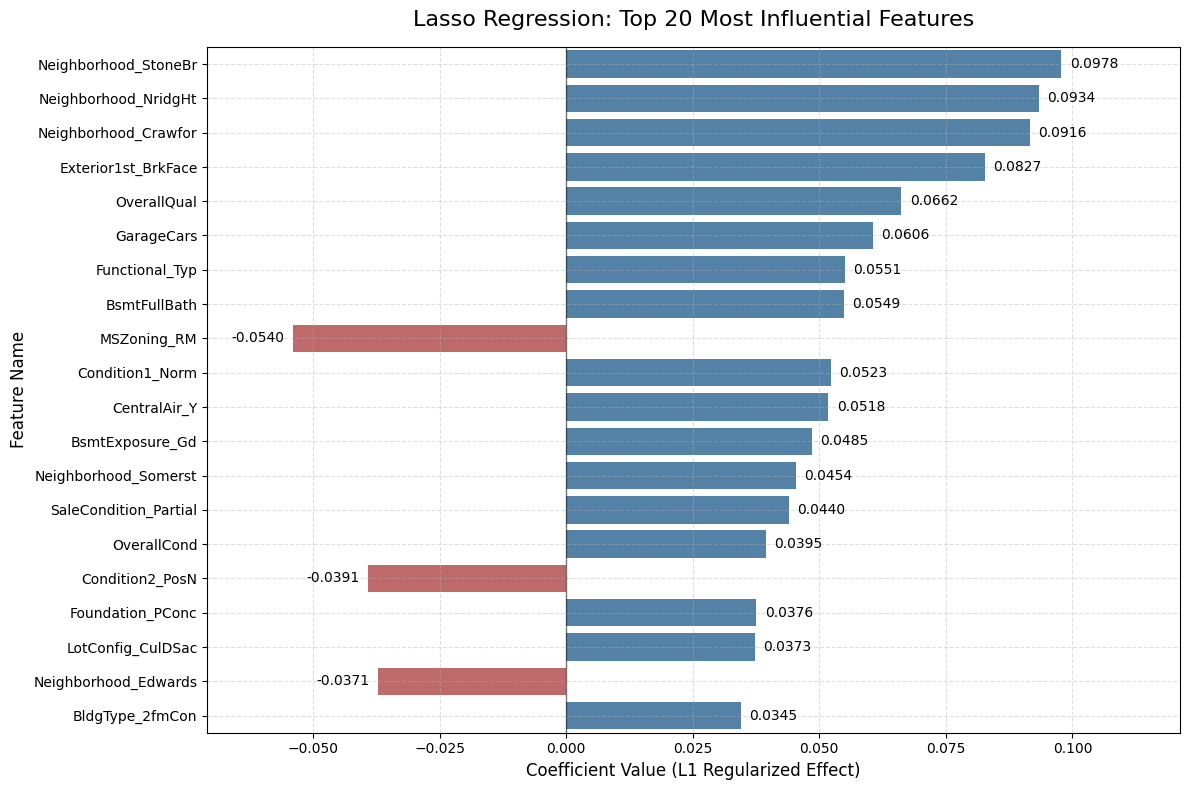
\includegraphics[width=0.9\columnwidth]{../picture/Lasso_influential_features_withoutSD.png}
        \label{fig:lasso_before}
    }
    
    \vspace{0.2cm} % 兩張圖之間的垂直間距
    
    % 第二張圖：轉換後
    \subfigure[After: Yeo-Johnson Transformed Lasso (Aligned with GBR)]{
        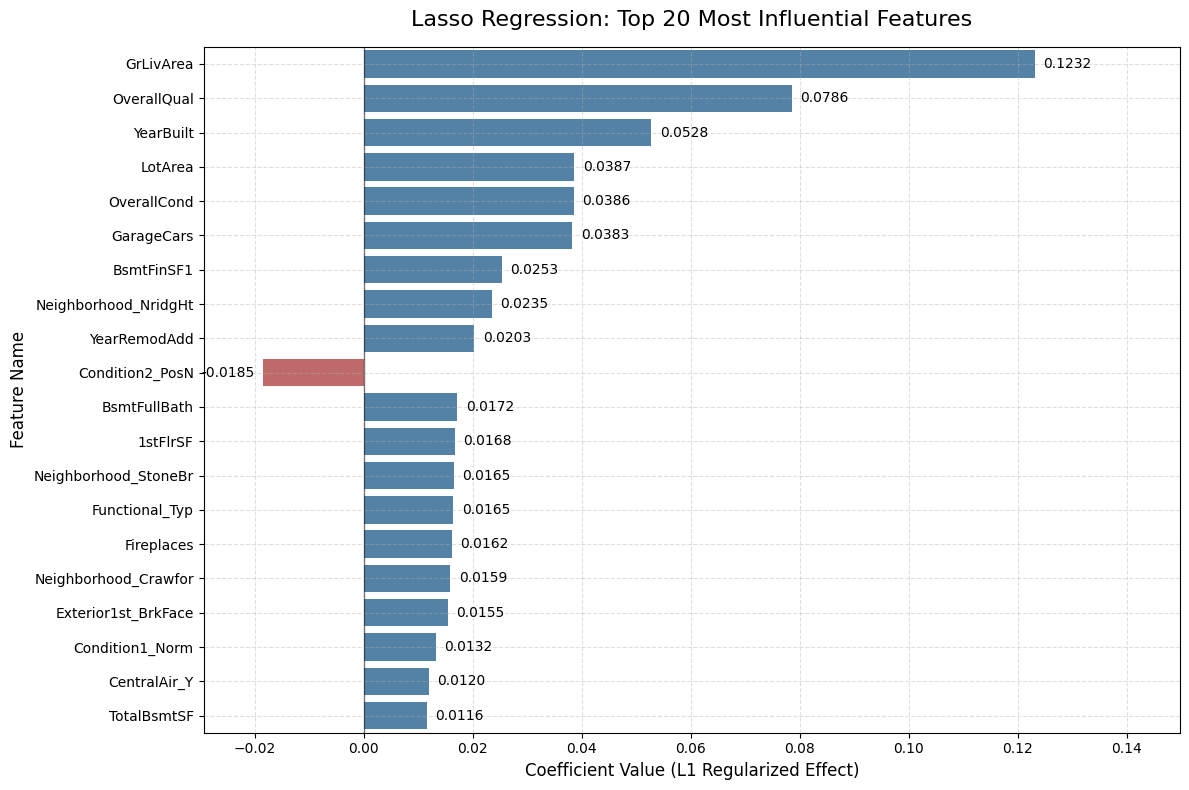
\includegraphics[width=0.9\columnwidth]{../picture/lasso_influential_features.png}
        \label{fig:lasso_after}
    }
    
    \caption{Comparison of Lasso feature importance before and after resolving scale distortion and non-normality.}
    \label{fig:feature_transformation}
\end{figure}

\begin{table}[htbp]
\centering
\caption{Impact of Feature Transformation on Model Performance (CV RMSE)}
\label{tab:transformation_impact}
% 使用 resizebox 將表格寬度限制在當前欄寬 (\columnwidth)
\resizebox{\columnwidth}{!}{%
\begin{tabular}{@{}lccc@{}}
\toprule
\textbf{Strategy}               & \textbf{Baseline} & \textbf{Lasso}  & \textbf{Ridge}  \\ \midrule
Unstandardized                  & 0.1657            & 0.1445          & 0.1426          \\
StandardScaler Only             & 0.1636            & 0.1480          & 0.1437          \\
\textbf{Yeo-Johnson Transform}  & \textbf{0.1501}   & \textbf{0.1323} & \textbf{0.1346} \\ \bottomrule
\end{tabular}%
}
\end{table}

\subsection{Model Interpretability: Diagnosing Counterintuitive Coefficients}

Even after the Yeo-Johnson transformation optimized our regularized models, a granular inspection of the feature importance revealed counterintuitive predictive behaviors. For instance, the linear models assigned a negative weight to feature \texttt{Condition2\_PosN} (proximity to a park or greenbelt), paradoxically implying that beneficial neighborhood amenities decrease home value.

As empirical evidence of this vulnerability, we traced this specific coefficient back to its raw training instances (Table \ref{tab:outlier_diagnosis}). We discovered that this algorithmic anomaly was driven by a combination of categorical sparsity and isolated outliers. Datapoint Id 524 represents a massive anomaly: despite boasting the maximum \texttt{OverallQual} score of 10 and a sprawling \texttt{GrLivArea} of 4,676 sq.ft., its sale price is severely depressed at \$184,750. 

\begin{table}[htbp]
\centering
\caption{Diagnosis of Outlier-Induced Weight Distortion}
\label{tab:outlier_diagnosis}
% 使用 resizebox 將表格寬度限制在當前欄寬 (\columnwidth)
\resizebox{\columnwidth}{!}{%
\begin{tabular}{@{}lcccccc@{}}
\toprule
\textbf{Id} & \textbf{SalePrice} & \textbf{Neighborhood} & \textbf{OverallQual} & \textbf{GrLivArea} & \textbf{Cond.1} & \textbf{Cond.2} \\ \midrule
524         & \$184,750          & Edwards               & 10                   & 4,676              & PosN            & PosN            \\
826         & \$385,000          & NridgHt               & 10                   & 2,084              & PosN            & PosN            \\ \bottomrule
\end{tabular}%
}
\end{table}

Because the \texttt{PosN} condition is extremely sparse within the dataset, the global linear model was forced to disproportionately punish this specific feature weight to mathematically accommodate the localized price collapse of this single outlier. 

This empirical finding exposed a residual vulnerability in global linear models: their extreme susceptibility to localized noise within sparse features. This diagnosis served as the final catalyst for our transition to advanced tree-based ensembles. Unlike linear models, algorithms like the Gradient Boosting Regressor (GBR) and XGBoost can effectively isolate such anomalous datapoints into deep, specific splits, preventing localized noise from distorting the global feature logic.

\subsection{Hyperparameter Optimization: From Grid to Stochastic Search}

The performance of a Gradient Boosting Regressor (GBR) is highly sensitive to its hyperparameter configuration. To systematically identify an effective model structure, we initially employed a \textbf{Grid Search Cross-Validation (GridSearchCV)}. The search space was defined across four critical dimensions governing the ensemble's learning dynamics and tree architecture (Table \ref{tab:grid_search}). 

\begin{table}[htbp]
    \centering
    \renewcommand{\arraystretch}{1.2}
    % 使用 resizebox 確保不超出欄寬
    \resizebox{\columnwidth}{!}{%
    \begin{tabular}{llc}
        \toprule
        \textbf{Hyperparameter} & \textbf{Search Space} & \textbf{Best Parameter} \\
        \midrule
        \texttt{n\_estimators} & [500, 1000] & 1000 \\
        \texttt{learning\_rate} & [0.01, 0.05, 0.1] & 0.05 \\
        \texttt{max\_depth}    & [3, 4, 5] & 3 \\
        \texttt{subsample}     & [0.8, 0.9] & 0.9 \\
        \bottomrule 
    \end{tabular}%
    }
    \caption{GridSearchCV parameter space and optimal configuration.}
    \label{tab:grid_search}
\end{table}

Despite yielding a strong Cross-Validation RMSE of 0.1264, relying on GridSearchCV presents notable theoretical and computational limitations. Because Grid Search operates strictly on discrete, predefined intervals, it suffers from an inherent "blind spot" effect—it cannot guarantee finding the true global optimum if the ideal parameter values lie between the specified grid points. Furthermore, exhaustive search scales poorly with dimensionality. Evaluating our specified grid required computing 36 distinct configurations (180 total fits across 5 folds), which incurs substantial computational cost and limits our ability to expand search boundaries. 

To comprehensively address the "blind spot" and the combinatorial explosion of the discrete grid, we subsequently transitioned to \textbf{RandomizedSearchCV}. The true advantage of this stochastic optimization lies in its ability to sample from continuous probability distributions rather than being confined to a finite list of predefined values (Table \ref{tab:random_search_params}).

\begin{table}[htbp]
    \centering
    \renewcommand{\arraystretch}{1.2}
    \resizebox{\columnwidth}{!}{%
    \begin{tabular}{llc}
        \toprule
        \textbf{Hyperparameter} & \textbf{Search Range} & \textbf{Best Parameter} \\
        \midrule
        \texttt{n\_estimators}       & [300, 1500]  & 1308 \\
        \texttt{learning\_rate}      & [0.01, 0.10] & 0.0243 \\
        \texttt{max\_depth}          & [3, 8]       & 3 \\
        \texttt{subsample}           & [0.6, 1.0]   & 0.7246 \\
        \texttt{min\_samples\_split} & [2, 20]      & 16 \\
        \texttt{min\_samples\_leaf}  & [1, 10]      & 5 \\
        \bottomrule
    \end{tabular}%
    }
    \caption{RandomizedSearchCV parameter distributions and the identified optimal configuration.}
    \label{tab:random_search_params}
\end{table}

Beyond achieving higher predictive accuracy, RandomizedSearchCV demonstrated superior computational efficiency. While the exhaustive Grid Search evaluated 180 total fits to cover its sparse grid, the Randomized Search was explicitly constrained to only 100 iterations. By sampling intelligently from continuous distributions, the model successfully located a more optimal global minimum using significantly fewer computational resources.

\begin{table}[htbp]
    \centering
    \renewcommand{\arraystretch}{1.2}
    \resizebox{\columnwidth}{!}{%
    \begin{tabular}{lccc}
        \toprule
        \textbf{Optimization Strategy} & \textbf{CV RMSE} & \textbf{Test RMSE} & \textbf{MPE} \\
        \midrule
        GBR (Grid Search) & 0.1264 & 0.1353 & 14.49\% \\
        \textbf{GBR (Random Search)} & \textbf{0.1237} & \textbf{0.1321} & \textbf{14.13\%} \\
        \bottomrule
    \end{tabular}%
    }
    \caption{Performance comparison between Grid Search and Randomized Search optimization.}
    \label{tab:hyperparam_performance_comparison}
\end{table}

As demonstrated in Table \ref{tab:hyperparam_performance_comparison}, RandomizedSearchCV undeniably yields superior predictive performance. However, this observation naturally prompts a deeper analytical question: \textit{how exactly were these optimal hyperparameters derived, and why does this specific continuous combination outperform the discrete grid search results?}

\subsection{Validation Curve Analysis \& Stress Testing}

To empirically validate our stochastic search results and understand the model's structural boundaries, we conducted extreme stress testing across all six primary hyperparameters via validation curves (Figure \ref{fig:all_validation_curves}). Rather than merely confirming standard bias-variance tradeoffs (e.g., the U-shaped curves of \texttt{learning\_rate} and \texttt{max\_depth}), this stress testing yielded three profound insights into the ensemble's internal topology:

\begin{figure}[H]
    \centering
    
    % 第一排：樹的數量與學習率
    \subfigure[Number of Estimators]{
        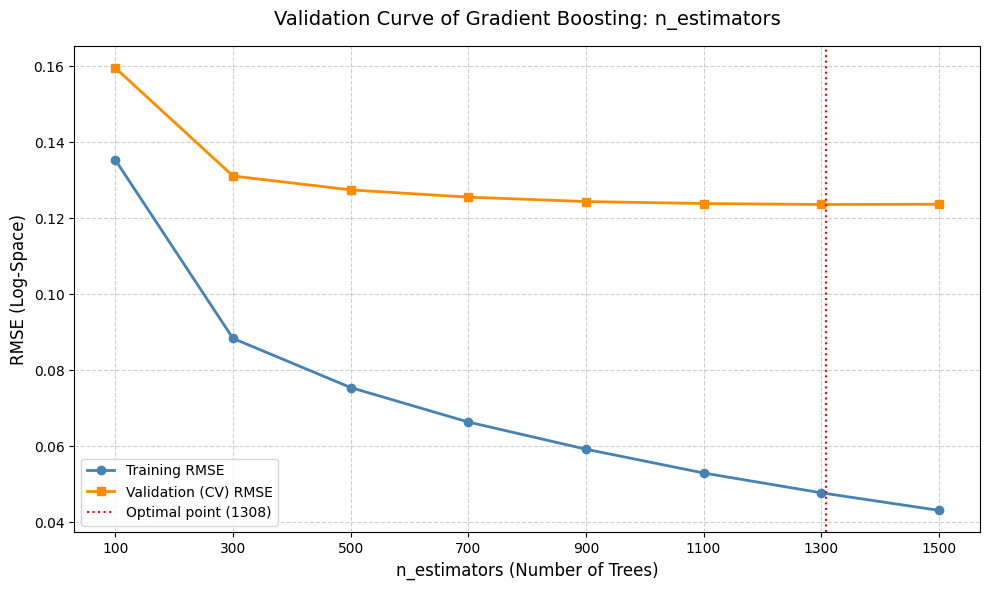
\includegraphics[width=0.45\columnwidth]{../picture/GB_n_estimater.png}
        \label{fig:vc_n_estimators}
    }\hfill
    \subfigure[Learning Rate]{
        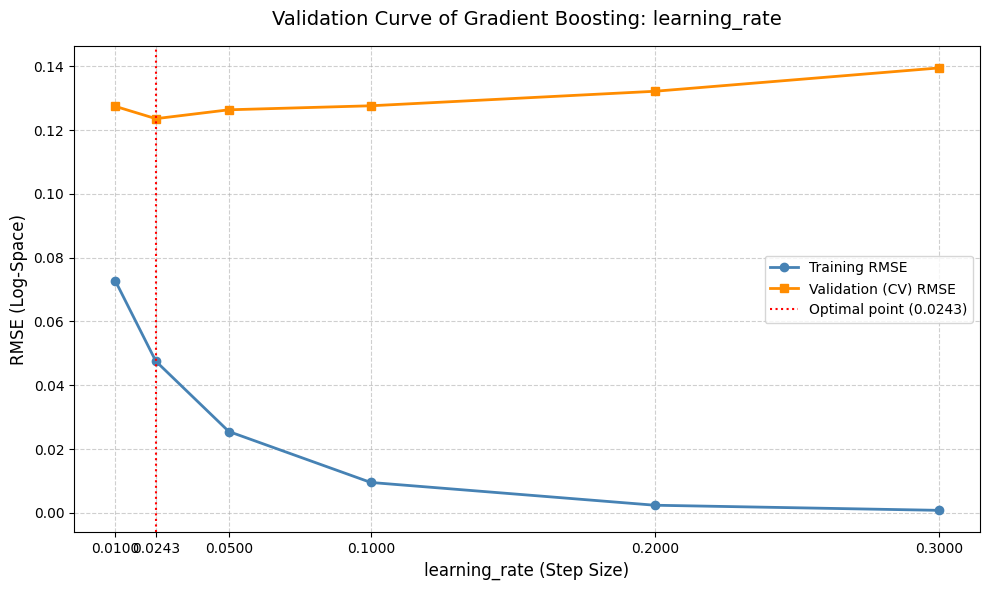
\includegraphics[width=0.45\columnwidth]{../picture/GB_learning_rate.png}
        \label{fig:vc_lr}
    }
    
    \vspace{-0.2cm} % 壓縮排與排之間的垂直間距，節省版面
    
    % 第二排：最大深度與抽樣比例
    \subfigure[Maximum Depth]{
        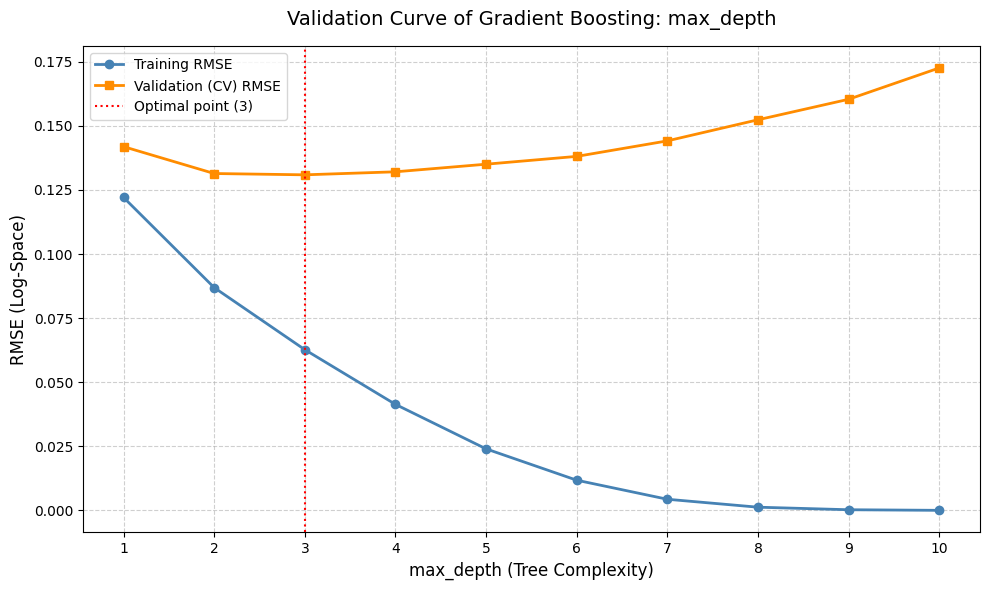
\includegraphics[width=0.45\columnwidth]{../picture/GB_max_depth.png}
        \label{fig:vc_max_depth}
    }\hfill
    \subfigure[Subsample Ratio]{
        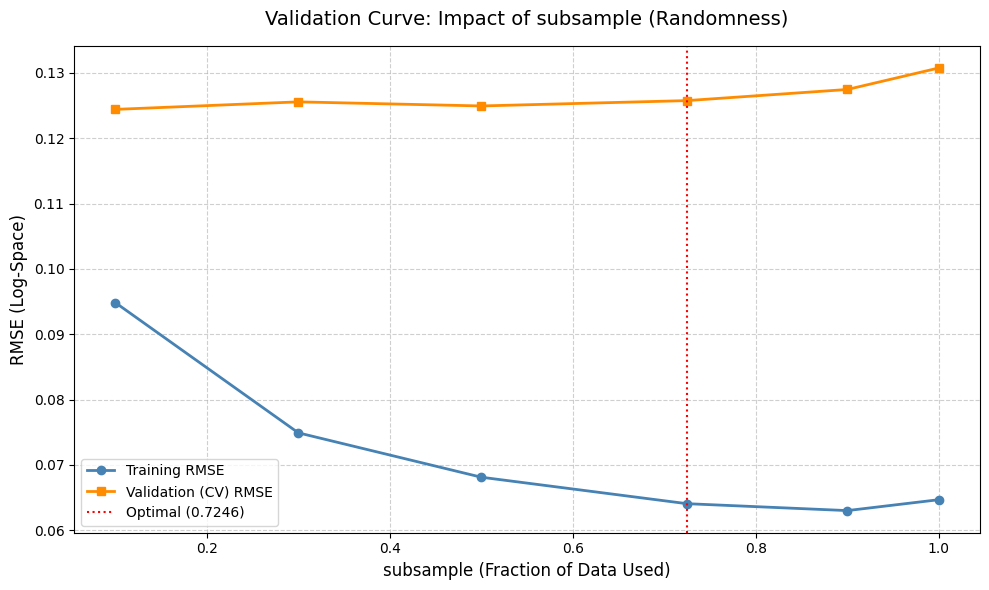
\includegraphics[width=0.45\columnwidth]{../picture/GB_sub_sample.png}
        \label{fig:vc_subsample}
    }
    
    \vspace{-0.2cm} % 壓縮排與排之間的垂直間距
    
    % 第三排：分裂與葉節點限制
    \subfigure[Min Samples Split]{
        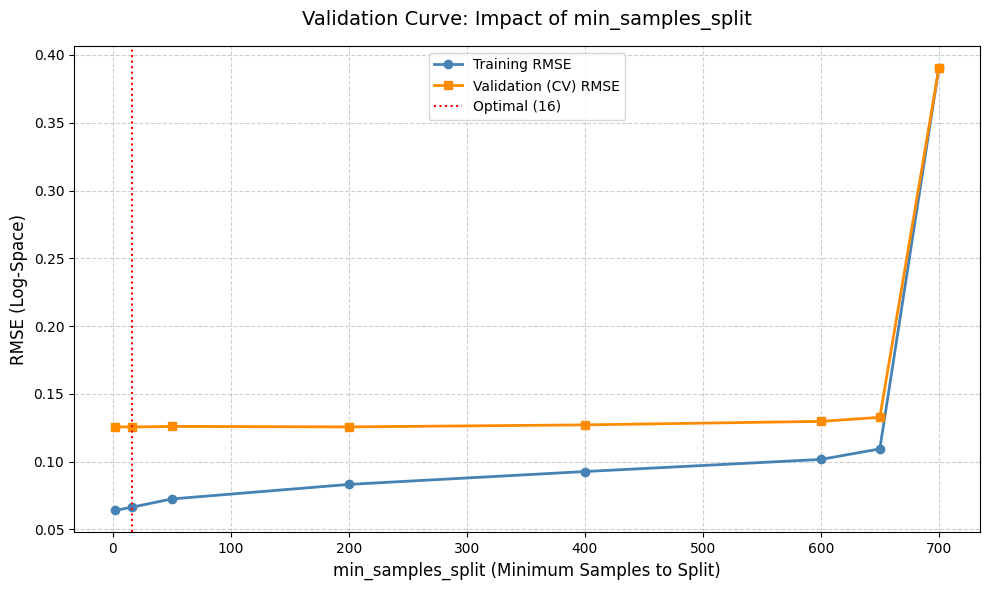
\includegraphics[width=0.45\columnwidth]{../picture/GB_min_sample_split.png}
        \label{fig:vc_min_split}
    }\hfill
    \subfigure[Min Samples Leaf]{
        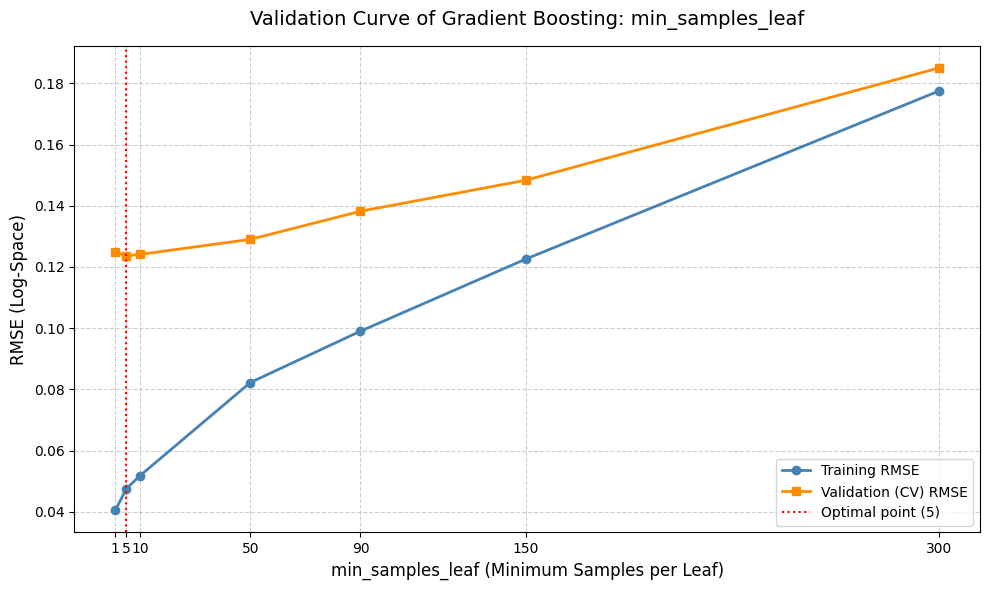
\includegraphics[width=0.45\columnwidth]{../picture/GB_min_sample_leaf.png}
        \label{fig:vc_min_leaf}
    }
    
    \caption{Validation curves for the six key hyperparameters of the Gradient Boosting Regressor. The blue line represents the Training RMSE, while the orange line indicates the Validation (CV) RMSE. Vertical dotted lines mark the optimal parameters identified by the tuning process.}
    \label{fig:all_validation_curves}
\end{figure}

\textbf{(1) Diminishing Returns vs. Computational Budget:} 
The cross-validation error minimized at \texttt{n\_estimators = 1308}. While the curve revealed a distinct plateau after 700 trees (indicating diminishing marginal returns on irreducible noise), the small scale of our dataset rendered the computational overhead negligible. Thus, we retained the full 1308 estimators to strictly maximize precision.

\textbf{(2) The Necessity of Stochastic Regularization:} 
Testing the \texttt{subsample} ratio validated the mathematical necessity of Stochastic Gradient Boosting. Dropping the ratio below 0.3 caused severe underfitting due to information deficit. Conversely, forcing \texttt{subsample = 1.0} disabled stochastic sampling, causing highly correlated trees to collectively memorize noise. The \texttt{RandomizedSearchCV} correctly converged on a "sweet spot" of 0.7246, optimally balancing structural housing information retention with stochastic noise protection.

\textbf{(3) Destructive Testing \& Topological Limits:} 
The most critical insights emerged from stress-testing the node constraints. At \texttt{max\_depth = 3}, a symmetric tree contains up to 8 leaves, yielding a theoretical average capacity of 146 samples per leaf ($1168 \div 8$). Setting \texttt{min\_samples\_leaf} beyond this limit (e.g., 150) triggered observable upward error inflections, and an aggressive threshold of 300 mathematically obliterated the depth-3 advantage ($1168 \div 300 \approx 3.89$ leaves maximum), causing catastrophic underfitting. Similarly, \texttt{min\_samples\_split} exhibited a sudden collapse at 700, reverse-engineering the fact that the maximum sample mass of our primary root nodes lies between 650 and 700. This destructive testing mathematically justifies our final permissive configurations (\texttt{leaf=5}, \texttt{split=16}), which provide essential regularization without paralyzing the tree's fundamental architecture.

\subsection{Architectural Synthesis: From Hybrid to Stacking}

While the Gradient Boosting Regressor (GBR) demonstrated strong individual performance, it suffers from a fundamental limitation inherent to tree-based models: the lack of \textbf{extrapolation capability}. Because decision trees partition the feature space into constant leaf values, they cannot inherently predict values beyond the maximum price encountered in the training set. To mitigate this, we initially implemented a \textbf{Hybrid Ensemble} by blending our regularized Lasso model with GBR. Using cross-validation, we performed a grid search across a range of blending ratios (from 1:0 to 0:1) to identify the optimal weight distribution between linear trends and non-linear nuances.

Subsequently, we transitioned to a formal \textbf{Stacking Architecture} to allow the model to autonomously learn the optimal combination of expert predictions. We evaluated three baseline configurations: (Lasso + Ridge + GBR), (Lasso + GBR), and (Ridge + GBR). Interestingly, our results indicated that all three combinations yielded near-identical test errors. This empirical finding confirms that Lasso and Ridge, both belonging to the linear paradigm, offer redundant inductive biases; thus, shifting weights between them does not contribute to additional predictive gain.

\subsection{The Final Frontier: Integrating XGBoost}

To further push the performance boundary, we integrated \textbf{XGBoost} into our ensemble. Unlike standard GBR, XGBoost incorporates advanced L1 and L2 regularization directly into its objective function, making it superior at handling the high-dimensional sparsity present in the Ames dataset. In our final architectural optimization, we pruned the redundant Ridge model and established a three-pillar Stacking framework comprising \textbf{Lasso, GBR, and XGBoost}. This synthesis successfully leveraged Lasso's global anchoring with the dual tree-based models' mastery of non-linear interactions, ultimately achieving our most robust and precise predictive performance.

\end{document}

\subsection{從未標準化到yeo-johnson}
在經過數居處理後，我們便開始使用 baseline lasso ridge 以及 GBR 模型，但我們發現線性模型(Lasso and Ridge) 與 GBR 模型間對於特徵的重要性有出路，線性模型更重視Neighborhood ，而 GBR 重視房子的整體狀況，後來發現是因為數據並未標準化，對於線性模型來說，若未標準化，由於 Neighborhood 經過one hot encoding，因此模型會給這類feature 較大的權重，然而經過標準化後，我們發現，其結果不如未標準化的結果，因此我們導入 yeo-johnson ，將具有高度偏態的 features 常態化，結果便優於未標準化的結果，且 features 的重要性也與 GBR 一致。


\subsection{從 GBR Hybrid 到 Stacking}
其實從結果來看 GBR 以表現很好了，然而畢竟 GBR 樹狀模型，樹狀模型的局限便是無法推理高於最高房價的房子(例如資料及的最高房價為 20 萬美金，擇期上限僅能預測到此金額)，而線性模型便可補足此問題，因此我們後續將最好的線性模型 Lasso 與 GBR 混合，並利用 Cross validation 1:0 = lasso : GBR 到 0:1 = lasso : GBR ，比較出最好比例的混合模型。後續我們更導入 stacking 由模型自行去尋找權重，我們分別嘗試三總組合(Lasso + Ridge + GBR), (Lasso + GBR), (Ridge + GBR)，然而結果顯示三長的 test error 都完全相同，主要是 lasso 與 Ridge 皆為線性模型，所以僅有模型間權重的差異，並不會改變整體的表現性